% Options for packages loaded elsewhere
\PassOptionsToPackage{unicode}{hyperref}
\PassOptionsToPackage{hyphens}{url}
%
\documentclass[
]{article}
\usepackage{lmodern}
\usepackage{amssymb,amsmath}
\usepackage{ifxetex,ifluatex}
\ifnum 0\ifxetex 1\fi\ifluatex 1\fi=0 % if pdftex
  \usepackage[T1]{fontenc}
  \usepackage[utf8]{inputenc}
  \usepackage{textcomp} % provide euro and other symbols
\else % if luatex or xetex
  \usepackage{unicode-math}
  \defaultfontfeatures{Scale=MatchLowercase}
  \defaultfontfeatures[\rmfamily]{Ligatures=TeX,Scale=1}
\fi
% Use upquote if available, for straight quotes in verbatim environments
\IfFileExists{upquote.sty}{\usepackage{upquote}}{}
\IfFileExists{microtype.sty}{% use microtype if available
  \usepackage[]{microtype}
  \UseMicrotypeSet[protrusion]{basicmath} % disable protrusion for tt fonts
}{}
\makeatletter
\@ifundefined{KOMAClassName}{% if non-KOMA class
  \IfFileExists{parskip.sty}{%
    \usepackage{parskip}
  }{% else
    \setlength{\parindent}{0pt}
    \setlength{\parskip}{6pt plus 2pt minus 1pt}}
}{% if KOMA class
  \KOMAoptions{parskip=half}}
\makeatother
\usepackage{xcolor}
\IfFileExists{xurl.sty}{\usepackage{xurl}}{} % add URL line breaks if available
\IfFileExists{bookmark.sty}{\usepackage{bookmark}}{\usepackage{hyperref}}
\hypersetup{
  pdftitle={Reproducible Research: Project 1},
  pdfauthor={lnma},
  hidelinks,
  pdfcreator={LaTeX via pandoc}}
\urlstyle{same} % disable monospaced font for URLs
\usepackage[margin=1in]{geometry}
\usepackage{color}
\usepackage{fancyvrb}
\newcommand{\VerbBar}{|}
\newcommand{\VERB}{\Verb[commandchars=\\\{\}]}
\DefineVerbatimEnvironment{Highlighting}{Verbatim}{commandchars=\\\{\}}
% Add ',fontsize=\small' for more characters per line
\usepackage{framed}
\definecolor{shadecolor}{RGB}{248,248,248}
\newenvironment{Shaded}{\begin{snugshade}}{\end{snugshade}}
\newcommand{\AlertTok}[1]{\textcolor[rgb]{0.94,0.16,0.16}{#1}}
\newcommand{\AnnotationTok}[1]{\textcolor[rgb]{0.56,0.35,0.01}{\textbf{\textit{#1}}}}
\newcommand{\AttributeTok}[1]{\textcolor[rgb]{0.77,0.63,0.00}{#1}}
\newcommand{\BaseNTok}[1]{\textcolor[rgb]{0.00,0.00,0.81}{#1}}
\newcommand{\BuiltInTok}[1]{#1}
\newcommand{\CharTok}[1]{\textcolor[rgb]{0.31,0.60,0.02}{#1}}
\newcommand{\CommentTok}[1]{\textcolor[rgb]{0.56,0.35,0.01}{\textit{#1}}}
\newcommand{\CommentVarTok}[1]{\textcolor[rgb]{0.56,0.35,0.01}{\textbf{\textit{#1}}}}
\newcommand{\ConstantTok}[1]{\textcolor[rgb]{0.00,0.00,0.00}{#1}}
\newcommand{\ControlFlowTok}[1]{\textcolor[rgb]{0.13,0.29,0.53}{\textbf{#1}}}
\newcommand{\DataTypeTok}[1]{\textcolor[rgb]{0.13,0.29,0.53}{#1}}
\newcommand{\DecValTok}[1]{\textcolor[rgb]{0.00,0.00,0.81}{#1}}
\newcommand{\DocumentationTok}[1]{\textcolor[rgb]{0.56,0.35,0.01}{\textbf{\textit{#1}}}}
\newcommand{\ErrorTok}[1]{\textcolor[rgb]{0.64,0.00,0.00}{\textbf{#1}}}
\newcommand{\ExtensionTok}[1]{#1}
\newcommand{\FloatTok}[1]{\textcolor[rgb]{0.00,0.00,0.81}{#1}}
\newcommand{\FunctionTok}[1]{\textcolor[rgb]{0.00,0.00,0.00}{#1}}
\newcommand{\ImportTok}[1]{#1}
\newcommand{\InformationTok}[1]{\textcolor[rgb]{0.56,0.35,0.01}{\textbf{\textit{#1}}}}
\newcommand{\KeywordTok}[1]{\textcolor[rgb]{0.13,0.29,0.53}{\textbf{#1}}}
\newcommand{\NormalTok}[1]{#1}
\newcommand{\OperatorTok}[1]{\textcolor[rgb]{0.81,0.36,0.00}{\textbf{#1}}}
\newcommand{\OtherTok}[1]{\textcolor[rgb]{0.56,0.35,0.01}{#1}}
\newcommand{\PreprocessorTok}[1]{\textcolor[rgb]{0.56,0.35,0.01}{\textit{#1}}}
\newcommand{\RegionMarkerTok}[1]{#1}
\newcommand{\SpecialCharTok}[1]{\textcolor[rgb]{0.00,0.00,0.00}{#1}}
\newcommand{\SpecialStringTok}[1]{\textcolor[rgb]{0.31,0.60,0.02}{#1}}
\newcommand{\StringTok}[1]{\textcolor[rgb]{0.31,0.60,0.02}{#1}}
\newcommand{\VariableTok}[1]{\textcolor[rgb]{0.00,0.00,0.00}{#1}}
\newcommand{\VerbatimStringTok}[1]{\textcolor[rgb]{0.31,0.60,0.02}{#1}}
\newcommand{\WarningTok}[1]{\textcolor[rgb]{0.56,0.35,0.01}{\textbf{\textit{#1}}}}
\usepackage{graphicx,grffile}
\makeatletter
\def\maxwidth{\ifdim\Gin@nat@width>\linewidth\linewidth\else\Gin@nat@width\fi}
\def\maxheight{\ifdim\Gin@nat@height>\textheight\textheight\else\Gin@nat@height\fi}
\makeatother
% Scale images if necessary, so that they will not overflow the page
% margins by default, and it is still possible to overwrite the defaults
% using explicit options in \includegraphics[width, height, ...]{}
\setkeys{Gin}{width=\maxwidth,height=\maxheight,keepaspectratio}
% Set default figure placement to htbp
\makeatletter
\def\fps@figure{htbp}
\makeatother
\setlength{\emergencystretch}{3em} % prevent overfull lines
\providecommand{\tightlist}{%
  \setlength{\itemsep}{0pt}\setlength{\parskip}{0pt}}
\setcounter{secnumdepth}{-\maxdimen} % remove section numbering

\title{Reproducible Research: Project 1}
\author{lnma}
\date{4/27/2020}

\begin{document}
\maketitle

\hypertarget{load-and-preprocess-data}{%
\subsection{Load and preprocess data}\label{load-and-preprocess-data}}

\begin{enumerate}
\def\labelenumi{\arabic{enumi}.}
\tightlist
\item
  Unzip data to csv file
\end{enumerate}

\begin{Shaded}
\begin{Highlighting}[]
\NormalTok{url <-}\StringTok{ "https://d396qusza40orc.cloudfront.net/repdata%2Fdata%2Factivity.zip"}
\NormalTok{destfile <-}\StringTok{ "step_data.zip"}
\KeywordTok{download.file}\NormalTok{(url, destfile)}
\KeywordTok{unzip}\NormalTok{(destfile)}
\end{Highlighting}
\end{Shaded}

\begin{enumerate}
\def\labelenumi{\arabic{enumi}.}
\setcounter{enumi}{1}
\tightlist
\item
  Load the data
\end{enumerate}

\begin{Shaded}
\begin{Highlighting}[]
\NormalTok{activity <-}\StringTok{ }\KeywordTok{read.csv}\NormalTok{(}\StringTok{"activity.csv"}\NormalTok{, }\DataTypeTok{sep =} \StringTok{","}\NormalTok{)}
\end{Highlighting}
\end{Shaded}

\begin{enumerate}
\def\labelenumi{\arabic{enumi}.}
\setcounter{enumi}{2}
\tightlist
\item
  Add a column of day that the first day is 2012-10-01
\end{enumerate}

\begin{Shaded}
\begin{Highlighting}[]
\NormalTok{activity}\OperatorTok{$}\NormalTok{date<-}\KeywordTok{as.Date}\NormalTok{(}\KeywordTok{as.character}\NormalTok{(activity}\OperatorTok{$}\NormalTok{date))}
\NormalTok{activity}\OperatorTok{$}\NormalTok{day<-activity}\OperatorTok{$}\NormalTok{date}\OperatorTok{-}\NormalTok{activity}\OperatorTok{$}\NormalTok{date[}\DecValTok{1}\NormalTok{]}\OperatorTok{+}\DecValTok{1}
\end{Highlighting}
\end{Shaded}

\begin{enumerate}
\def\labelenumi{\arabic{enumi}.}
\setcounter{enumi}{3}
\tightlist
\item
  Have a look at the data
\end{enumerate}

\begin{Shaded}
\begin{Highlighting}[]
\KeywordTok{str}\NormalTok{(activity)}
\end{Highlighting}
\end{Shaded}

\begin{verbatim}
## 'data.frame':    17568 obs. of  4 variables:
##  $ steps   : int  NA NA NA NA NA NA NA NA NA NA ...
##  $ date    : Date, format: "2012-10-01" "2012-10-01" ...
##  $ interval: int  0 5 10 15 20 25 30 35 40 45 ...
##  $ day     : 'difftime' num  1 1 1 1 ...
##   ..- attr(*, "units")= chr "days"
\end{verbatim}

\begin{Shaded}
\begin{Highlighting}[]
\KeywordTok{head}\NormalTok{(activity)}
\end{Highlighting}
\end{Shaded}

\begin{verbatim}
##   steps       date interval    day
## 1    NA 2012-10-01        0 1 days
## 2    NA 2012-10-01        5 1 days
## 3    NA 2012-10-01       10 1 days
## 4    NA 2012-10-01       15 1 days
## 5    NA 2012-10-01       20 1 days
## 6    NA 2012-10-01       25 1 days
\end{verbatim}

\hypertarget{what-is-mean-total-number-of-steps-taken-per-day}{%
\subsection{What is mean total number of steps taken per
day?}\label{what-is-mean-total-number-of-steps-taken-per-day}}

\begin{enumerate}
\def\labelenumi{\arabic{enumi}.}
\tightlist
\item
  Calculate the total number of steps taken per day
\end{enumerate}

\begin{Shaded}
\begin{Highlighting}[]
\NormalTok{totalStep_day<-}\KeywordTok{tapply}\NormalTok{(activity}\OperatorTok{$}\NormalTok{steps,activity}\OperatorTok{$}\NormalTok{day,sum,}\DataTypeTok{na.rm=}\OtherTok{TRUE}\NormalTok{)}
\end{Highlighting}
\end{Shaded}

\begin{enumerate}
\def\labelenumi{\arabic{enumi}.}
\setcounter{enumi}{1}
\tightlist
\item
  Barplot total number of steps taken for each day\\
  The mean and median values are plotted as red and blue lines
  respectively
\end{enumerate}

\begin{Shaded}
\begin{Highlighting}[]
\KeywordTok{barplot}\NormalTok{(totalStep_day,}\DataTypeTok{main=}\StringTok{'Total steps taken per day'}\NormalTok{,}
     \DataTypeTok{xlab =} \StringTok{'Day'}\NormalTok{,}\DataTypeTok{ylab=}\StringTok{'Total steps'}\NormalTok{)}
\KeywordTok{abline}\NormalTok{(}\DataTypeTok{h =} \KeywordTok{mean}\NormalTok{(totalStep_day), }\DataTypeTok{lty =} \DecValTok{1}\NormalTok{, }\DataTypeTok{lwd =} \DecValTok{1}\NormalTok{, }\DataTypeTok{col =} \StringTok{"red"}\NormalTok{)}
\KeywordTok{abline}\NormalTok{(}\DataTypeTok{h =} \KeywordTok{median}\NormalTok{(totalStep_day), }\DataTypeTok{lty =} \DecValTok{1}\NormalTok{, }\DataTypeTok{lwd =} \DecValTok{1}\NormalTok{, }\DataTypeTok{col =} \StringTok{"blue"}\NormalTok{)}
\KeywordTok{legend}\NormalTok{(}\StringTok{'top'}\NormalTok{,}\KeywordTok{c}\NormalTok{(}\StringTok{'Mean'}\NormalTok{,}\StringTok{'Median'}\NormalTok{),}\DataTypeTok{col=}\KeywordTok{c}\NormalTok{(}\StringTok{'red'}\NormalTok{,}\StringTok{'blue'}\NormalTok{),}\DataTypeTok{lty =} \KeywordTok{c}\NormalTok{(}\DecValTok{1}\NormalTok{,}\DecValTok{1}\NormalTok{),}\DataTypeTok{lwd=}\KeywordTok{c}\NormalTok{(}\DecValTok{1}\NormalTok{,}\DecValTok{1}\NormalTok{))}
\end{Highlighting}
\end{Shaded}

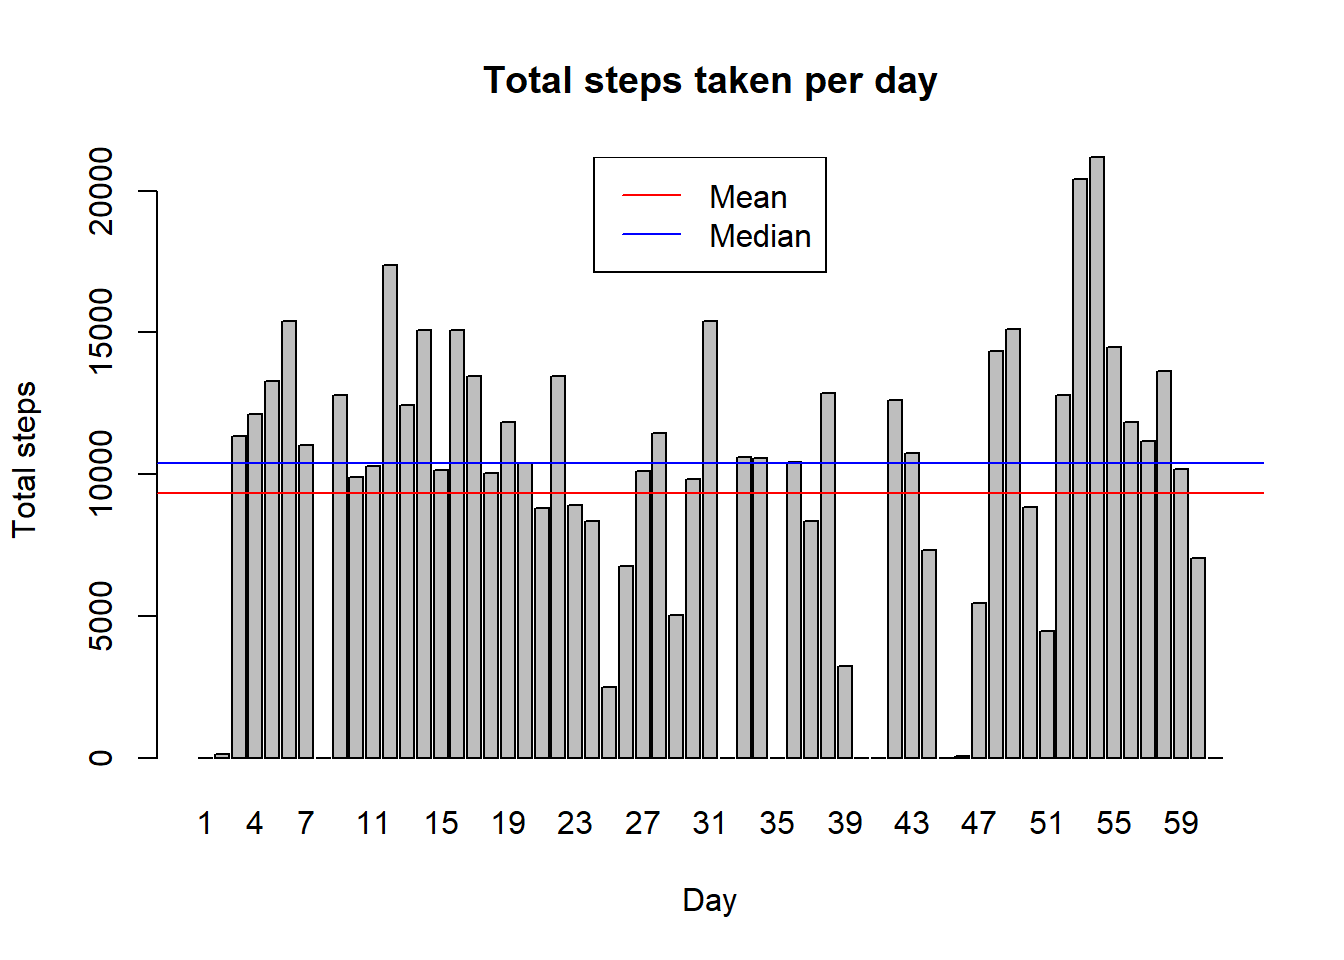
\includegraphics{PA1_template.Rmd_files/figure-latex/totalStep_day_bar-1.pdf}

\begin{enumerate}
\def\labelenumi{\arabic{enumi}.}
\setcounter{enumi}{2}
\tightlist
\item
  Histogram of total number of steps taken for each day\\
  The mean and median values are plotted as red and blue lines
  respectively
\end{enumerate}

\begin{Shaded}
\begin{Highlighting}[]
\KeywordTok{hist}\NormalTok{(totalStep_day,}\DataTypeTok{main=}\StringTok{'Total steps taken per day'}\NormalTok{,}
        \DataTypeTok{xlab =} \StringTok{'Total steps per day'}\NormalTok{,}\DataTypeTok{ylab=}\StringTok{'Frequency'}\NormalTok{)}
\CommentTok{#add lines of mean and median in red and blue respectively}
\KeywordTok{abline}\NormalTok{(}\DataTypeTok{v =} \KeywordTok{mean}\NormalTok{(totalStep_day), }\DataTypeTok{lty =} \DecValTok{1}\NormalTok{, }\DataTypeTok{lwd =} \DecValTok{1}\NormalTok{, }\DataTypeTok{col =} \StringTok{"red"}\NormalTok{)}
\KeywordTok{abline}\NormalTok{(}\DataTypeTok{v =} \KeywordTok{median}\NormalTok{(totalStep_day), }\DataTypeTok{lty =} \DecValTok{1}\NormalTok{, }\DataTypeTok{lwd =} \DecValTok{1}\NormalTok{, }\DataTypeTok{col =} \StringTok{"blue"}\NormalTok{)}
\KeywordTok{legend}\NormalTok{(}\StringTok{'topright'}\NormalTok{,}\KeywordTok{c}\NormalTok{(}\StringTok{'Mean'}\NormalTok{,}\StringTok{'Median'}\NormalTok{),}\DataTypeTok{col=}\KeywordTok{c}\NormalTok{(}\StringTok{'red'}\NormalTok{,}\StringTok{'blue'}\NormalTok{),}\DataTypeTok{lty =} \KeywordTok{c}\NormalTok{(}\DecValTok{1}\NormalTok{,}\DecValTok{1}\NormalTok{),}\DataTypeTok{lwd=}\KeywordTok{c}\NormalTok{(}\DecValTok{1}\NormalTok{,}\DecValTok{1}\NormalTok{))}
\end{Highlighting}
\end{Shaded}

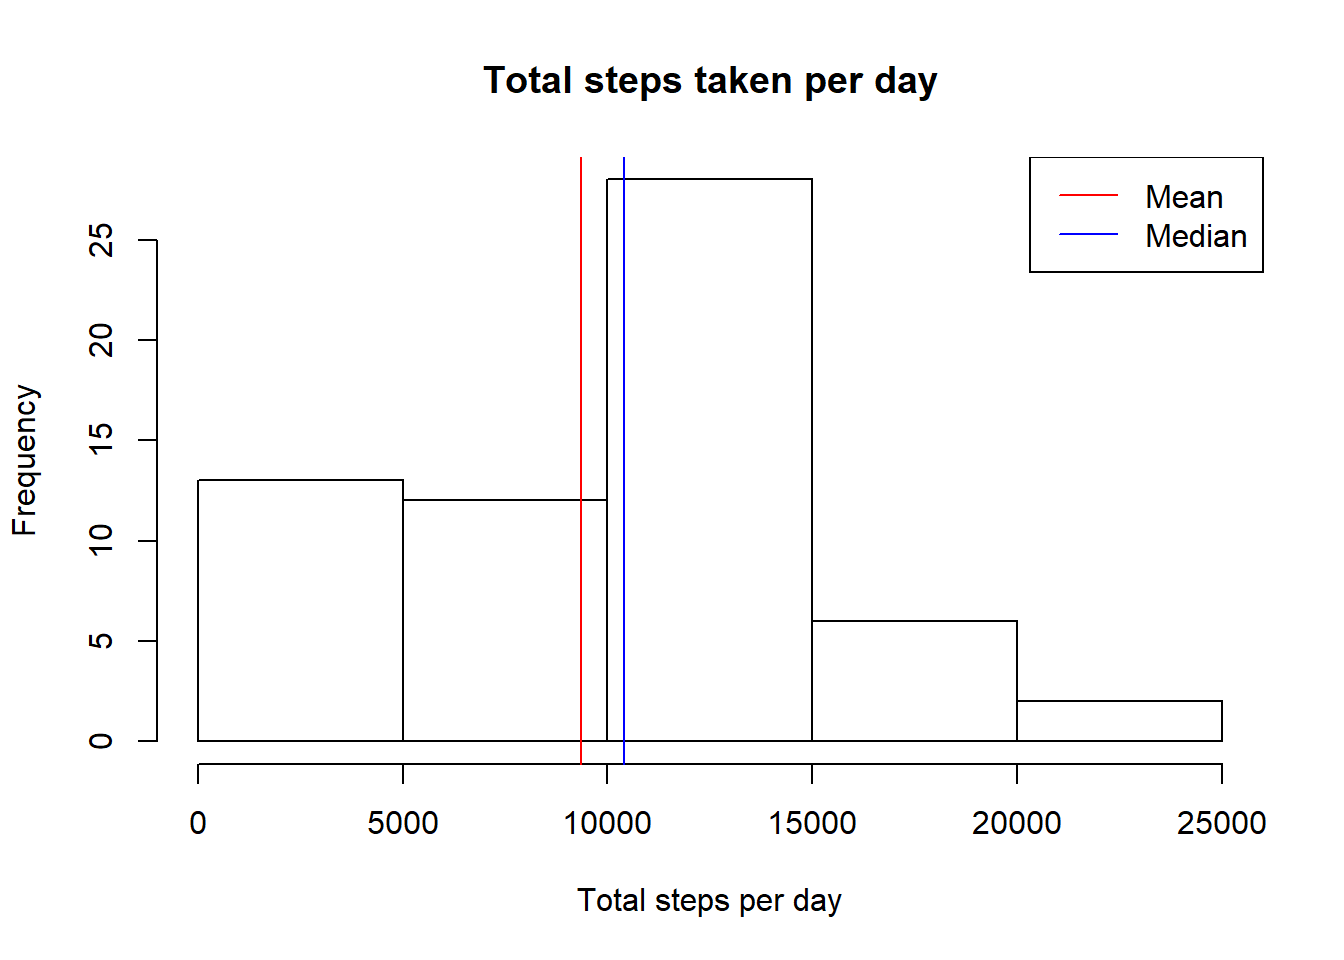
\includegraphics{PA1_template.Rmd_files/figure-latex/totalStep_day_hist-1.pdf}

\hypertarget{what-is-the-average-daily-activity-pattern}{%
\subsection{What is the average daily activity
pattern?}\label{what-is-the-average-daily-activity-pattern}}

\begin{enumerate}
\def\labelenumi{\arabic{enumi}.}
\tightlist
\item
  Calculate the average number of steps taken per interval
\end{enumerate}

\begin{Shaded}
\begin{Highlighting}[]
\NormalTok{avgStep_interval<-}\KeywordTok{tapply}\NormalTok{(activity}\OperatorTok{$}\NormalTok{steps,activity}\OperatorTok{$}\NormalTok{interval,mean,}\DataTypeTok{na.rm=}\OtherTok{TRUE}\NormalTok{)}
\end{Highlighting}
\end{Shaded}

\begin{enumerate}
\def\labelenumi{\arabic{enumi}.}
\setcounter{enumi}{1}
\tightlist
\item
  Make a time series plot of the 5-minute interval (x-axis) and the
  average number of steps taken, averaged across all days (y-axis), the
  maxium point is highlighted
\end{enumerate}

\begin{Shaded}
\begin{Highlighting}[]
\KeywordTok{plot}\NormalTok{(avgStep_interval,}\DataTypeTok{ty=}\StringTok{'l'}\NormalTok{,}\DataTypeTok{main=}\StringTok{'Average steps vs. daily time interval'}\NormalTok{,}
     \DataTypeTok{xlab =} \StringTok{'Daily time interval'}\NormalTok{,}\DataTypeTok{ylab =} \StringTok{'Average steps'}\NormalTok{)}
\CommentTok{#maximum average number of steps}
\NormalTok{x_max=}\KeywordTok{as.numeric}\NormalTok{(}\KeywordTok{which}\NormalTok{(avgStep_interval}\OperatorTok{==}\KeywordTok{max}\NormalTok{(avgStep_interval)))}
\NormalTok{y_max=}\KeywordTok{max}\NormalTok{(avgStep_interval)}
\NormalTok{p<-}\KeywordTok{c}\NormalTok{(}\KeywordTok{round}\NormalTok{(x_max),}\KeywordTok{round}\NormalTok{(y_max))}
\KeywordTok{points}\NormalTok{(}\KeywordTok{t}\NormalTok{(p),}\DataTypeTok{pch=}\DecValTok{8}\NormalTok{,}\DataTypeTok{col=}\StringTok{'red'}\NormalTok{,}\DataTypeTok{cex=}\DecValTok{2}\NormalTok{)}
\end{Highlighting}
\end{Shaded}

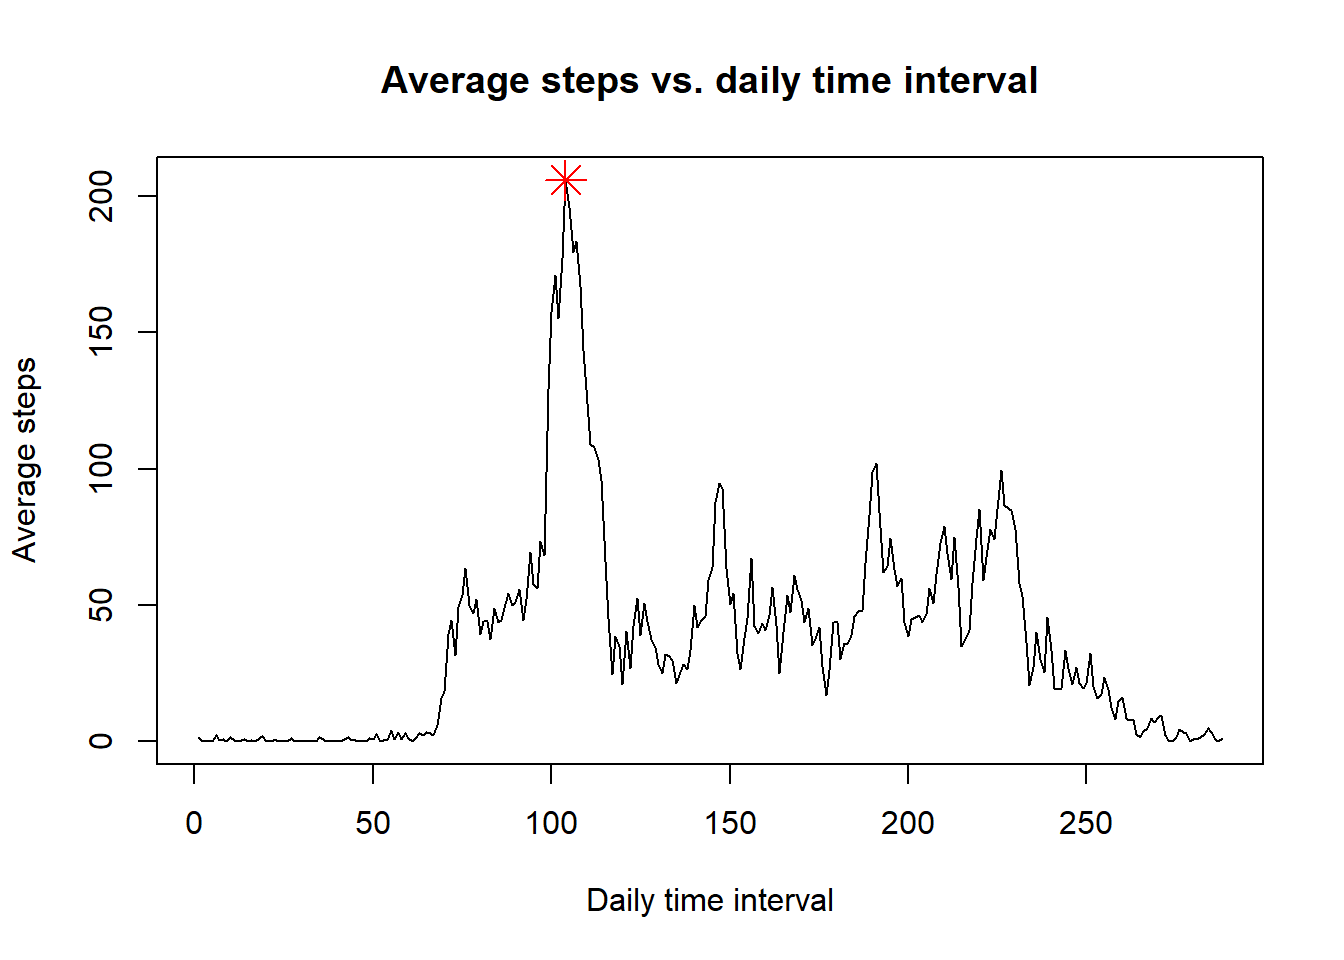
\includegraphics{PA1_template.Rmd_files/figure-latex/totalStep_day_plot-1.pdf}

3.Which 5-minute interval, on average across all the days in the
dataset, contains the maximum number of steps?\\
Interval (835) contains on average the maximum number of steps
(206.1698).

\begin{Shaded}
\begin{Highlighting}[]
\NormalTok{x_max=}\KeywordTok{which}\NormalTok{(avgStep_interval}\OperatorTok{==}\KeywordTok{max}\NormalTok{(avgStep_interval))}
\NormalTok{y_max=}\KeywordTok{max}\NormalTok{(avgStep_interval)}
\NormalTok{x_max}
\end{Highlighting}
\end{Shaded}

\begin{verbatim}
## 835 
## 104
\end{verbatim}

\begin{Shaded}
\begin{Highlighting}[]
\NormalTok{y_max}
\end{Highlighting}
\end{Shaded}

\begin{verbatim}
## [1] 206.1698
\end{verbatim}

\hypertarget{imputing-missing-values}{%
\subsection{Imputing missing values}\label{imputing-missing-values}}

1.Calculate and report the total number of missing values in the dataset

\begin{Shaded}
\begin{Highlighting}[]
\NormalTok{na_number_steps<-}\KeywordTok{sum}\NormalTok{(}\KeywordTok{is.na}\NormalTok{(activity}\OperatorTok{$}\NormalTok{steps))}
\NormalTok{na_number_steps}
\end{Highlighting}
\end{Shaded}

\begin{verbatim}
## [1] 2304
\end{verbatim}

\begin{enumerate}
\def\labelenumi{\arabic{enumi}.}
\setcounter{enumi}{1}
\tightlist
\item
  Devise a strategy for filling in all of the missing values in the
  dataset. The strategy uses the mean mean for that 5-minute interval.
\end{enumerate}

\begin{Shaded}
\begin{Highlighting}[]
\NormalTok{activity_day<-}\KeywordTok{split}\NormalTok{(activity,activity}\OperatorTok{$}\NormalTok{day)}
\NormalTok{avgStep_day<-}\KeywordTok{as.numeric}\NormalTok{(}\KeywordTok{tapply}\NormalTok{(activity}\OperatorTok{$}\NormalTok{steps,activity}\OperatorTok{$}\NormalTok{day,mean,}\DataTypeTok{na.rm=}\OtherTok{TRUE}\NormalTok{))}
\NormalTok{activity_NA<-}\KeywordTok{data.frame}\NormalTok{()}
\ControlFlowTok{for}\NormalTok{(i }\ControlFlowTok{in} \DecValTok{1}\OperatorTok{:}\KeywordTok{length}\NormalTok{(avgStep_day))\{}
        \ControlFlowTok{if}\NormalTok{ (}\KeywordTok{sum}\NormalTok{(}\OperatorTok{!}\KeywordTok{is.na}\NormalTok{(activity_day[[i]][,}\DecValTok{1}\NormalTok{]))}\OperatorTok{==}\DecValTok{0}\NormalTok{)\{}
\NormalTok{                activity_day[[i]]}\OperatorTok{$}\NormalTok{steps<-avgStep_interval}
\NormalTok{        \}}\ControlFlowTok{else} \ControlFlowTok{if}\NormalTok{(}\KeywordTok{sum}\NormalTok{(}\KeywordTok{is.na}\NormalTok{(activity_day[[i]]}\OperatorTok{$}\NormalTok{steps))}\OperatorTok{!=}\DecValTok{0}\NormalTok{)\{}
                \ControlFlowTok{for}\NormalTok{ (j }\ControlFlowTok{in} \DecValTok{1}\OperatorTok{:}\KeywordTok{length}\NormalTok{(activity_day[[i]]}\OperatorTok{$}\NormalTok{steps))\{}
\NormalTok{                        activity_day[[i]][j,}\DecValTok{1}\NormalTok{]<-avgStep_interval[j]}
\NormalTok{                \}}
\NormalTok{        \}}
\NormalTok{        activity_NA<-}\KeywordTok{rbind}\NormalTok{(activity_NA,activity_day[[i]])}
\NormalTok{\}}
\end{Highlighting}
\end{Shaded}

\begin{enumerate}
\def\labelenumi{\arabic{enumi}.}
\setcounter{enumi}{2}
\tightlist
\item
  Create a new dataset that is equal to the original dataset but with
  the missing data filled in.
\end{enumerate}

\begin{Shaded}
\begin{Highlighting}[]
\KeywordTok{head}\NormalTok{(activity_NA)}
\end{Highlighting}
\end{Shaded}

\begin{verbatim}
##       steps       date interval    day
## 1 1.7169811 2012-10-01        0 1 days
## 2 0.3396226 2012-10-01        5 1 days
## 3 0.1320755 2012-10-01       10 1 days
## 4 0.1509434 2012-10-01       15 1 days
## 5 0.0754717 2012-10-01       20 1 days
## 6 2.0943396 2012-10-01       25 1 days
\end{verbatim}

\begin{enumerate}
\def\labelenumi{\arabic{enumi}.}
\setcounter{enumi}{3}
\tightlist
\item
  Make a histogram of the total number of steps taken each day and
  Calculate and report the mean and median total number of steps taken
  per day. Do these values differ from the estimates from the first part
  of the assignment? What is the impact of imputing missing data on the
  estimates of the total daily number of steps?\\
  Barplot total number of steps taken for each day without NAs
\end{enumerate}

\begin{Shaded}
\begin{Highlighting}[]
\NormalTok{totalStep_NA<-}\KeywordTok{tapply}\NormalTok{(activity_NA}\OperatorTok{$}\NormalTok{steps,activity_NA}\OperatorTok{$}\NormalTok{day,sum,}\DataTypeTok{na.rm=}\OtherTok{TRUE}\NormalTok{)}
\KeywordTok{barplot}\NormalTok{(totalStep_NA,}\DataTypeTok{main=}\StringTok{'Total steps taken per day without NA'}\NormalTok{,}
        \DataTypeTok{xlab =} \StringTok{'Day'}\NormalTok{,}\DataTypeTok{ylab=}\StringTok{'Total steps'}\NormalTok{)}
\KeywordTok{abline}\NormalTok{(}\DataTypeTok{h =} \KeywordTok{mean}\NormalTok{(totalStep_NA), }\DataTypeTok{lty =} \DecValTok{1}\NormalTok{, }\DataTypeTok{lwd =} \DecValTok{1}\NormalTok{, }\DataTypeTok{col =} \StringTok{"red"}\NormalTok{)}
\KeywordTok{abline}\NormalTok{(}\DataTypeTok{h =} \KeywordTok{median}\NormalTok{(totalStep_NA), }\DataTypeTok{lty =} \DecValTok{2}\NormalTok{, }\DataTypeTok{lwd =} \DecValTok{1}\NormalTok{, }\DataTypeTok{col =} \StringTok{"blue"}\NormalTok{)}
\KeywordTok{legend}\NormalTok{(}\StringTok{'top'}\NormalTok{,}\KeywordTok{c}\NormalTok{(}\StringTok{'Mean'}\NormalTok{,}\StringTok{'Median'}\NormalTok{),}\DataTypeTok{col=}\KeywordTok{c}\NormalTok{(}\StringTok{'red'}\NormalTok{,}\StringTok{'blue'}\NormalTok{),}\DataTypeTok{lty =} \KeywordTok{c}\NormalTok{(}\DecValTok{1}\NormalTok{,}\DecValTok{2}\NormalTok{),}\DataTypeTok{lwd=}\KeywordTok{c}\NormalTok{(}\DecValTok{1}\NormalTok{,}\DecValTok{1}\NormalTok{))}
\end{Highlighting}
\end{Shaded}

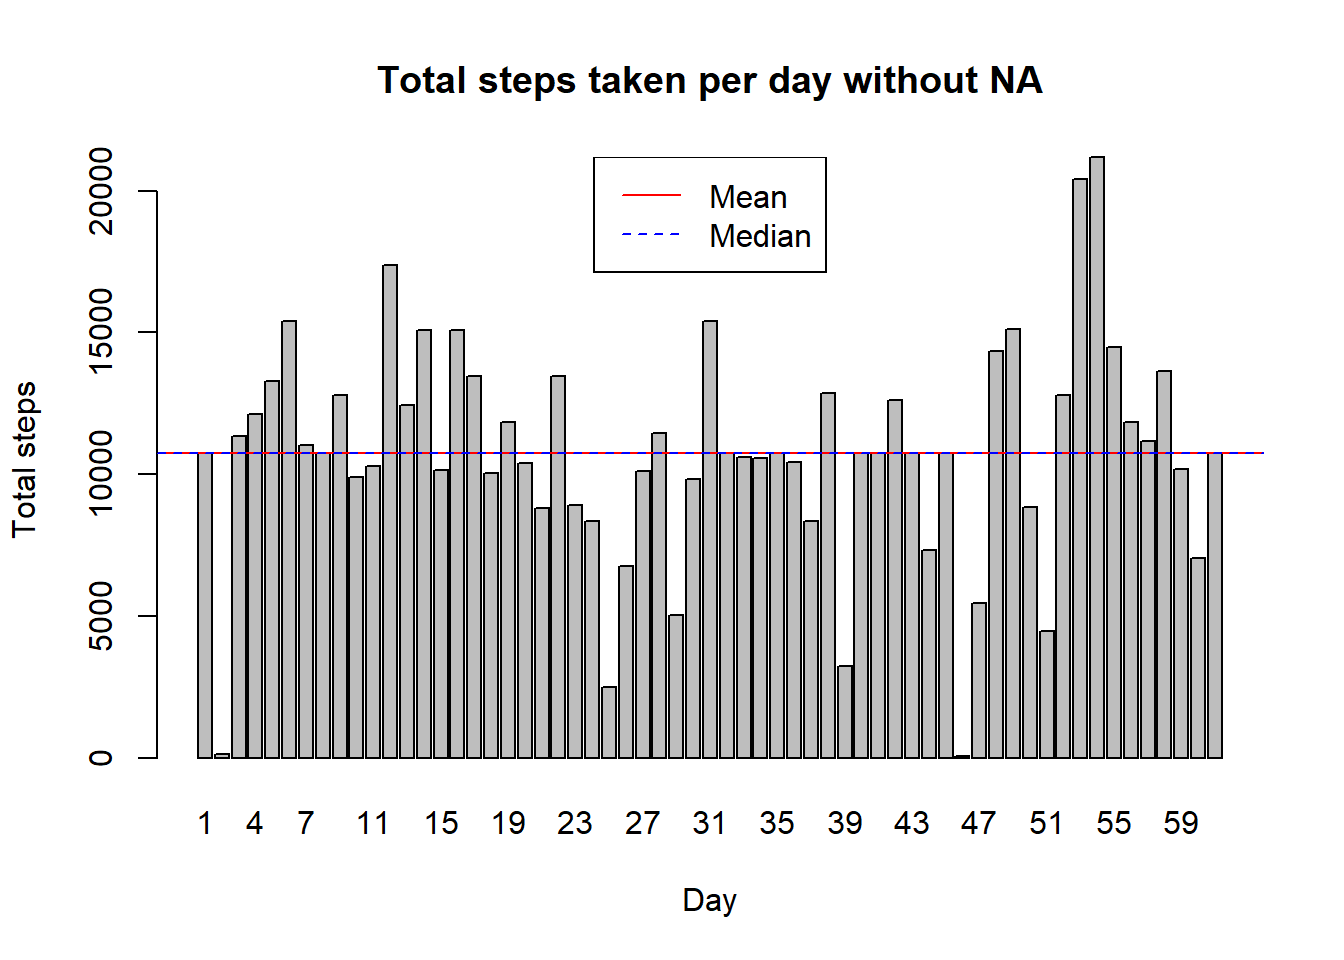
\includegraphics{PA1_template.Rmd_files/figure-latex/fill NA_barplot-1.pdf}

Histogram of total number of steps taken for each day without NAs

\begin{Shaded}
\begin{Highlighting}[]
\KeywordTok{hist}\NormalTok{(totalStep_NA,}\DataTypeTok{main=}\StringTok{'Total steps taken per day without NA'}\NormalTok{,}
        \DataTypeTok{xlab =} \StringTok{'Steps per day'}\NormalTok{,}\DataTypeTok{ylab=}\StringTok{'Frequency'}\NormalTok{)}
\KeywordTok{abline}\NormalTok{(}\DataTypeTok{v =} \KeywordTok{mean}\NormalTok{(totalStep_NA), }\DataTypeTok{lty =} \DecValTok{1}\NormalTok{, }\DataTypeTok{lwd =} \DecValTok{1}\NormalTok{, }\DataTypeTok{col =} \StringTok{"red"}\NormalTok{)}
\KeywordTok{abline}\NormalTok{(}\DataTypeTok{v =} \KeywordTok{median}\NormalTok{(totalStep_NA), }\DataTypeTok{lty =} \DecValTok{2}\NormalTok{, }\DataTypeTok{lwd =} \DecValTok{1}\NormalTok{, }\DataTypeTok{col =} \StringTok{"blue"}\NormalTok{)}
\KeywordTok{legend}\NormalTok{(}\StringTok{'top'}\NormalTok{,}\KeywordTok{c}\NormalTok{(}\StringTok{'Mean'}\NormalTok{,}\StringTok{'Median'}\NormalTok{),}\DataTypeTok{col=}\KeywordTok{c}\NormalTok{(}\StringTok{'red'}\NormalTok{,}\StringTok{'blue'}\NormalTok{),}\DataTypeTok{lty =} \KeywordTok{c}\NormalTok{(}\DecValTok{1}\NormalTok{,}\DecValTok{2}\NormalTok{),}\DataTypeTok{lwd=}\KeywordTok{c}\NormalTok{(}\DecValTok{1}\NormalTok{,}\DecValTok{1}\NormalTok{))}
\end{Highlighting}
\end{Shaded}

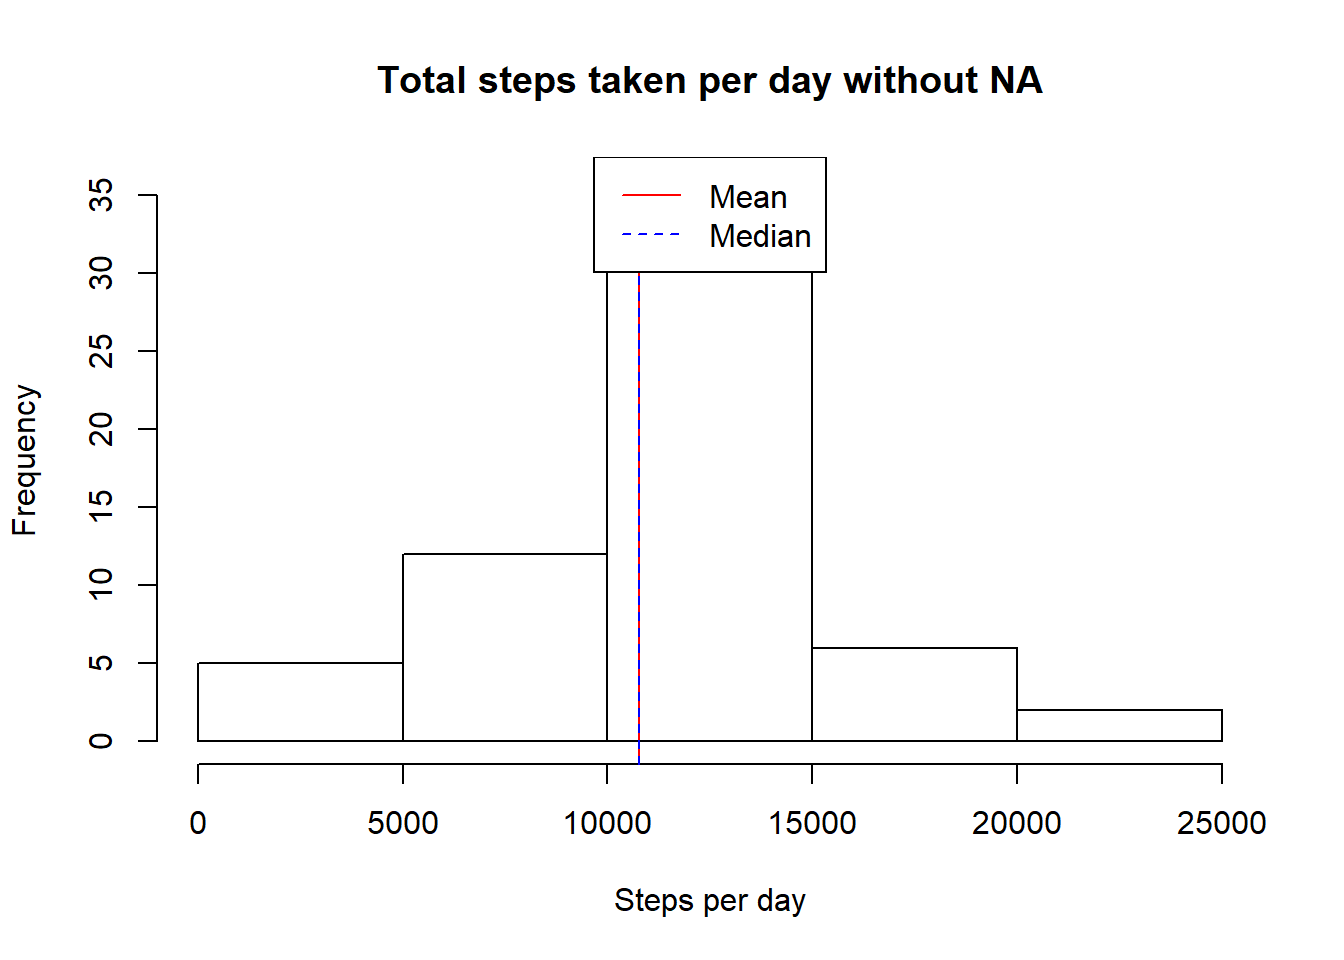
\includegraphics{PA1_template.Rmd_files/figure-latex/fill NA_hist-1.pdf}

Imputing missing values, mean of the total number of steps taken per day
increased while median decreased. The strategy leads to equal value of
mean and median of the total number of steps per day

\hypertarget{are-there-differences-in-activity-patterns-between-weekdays-and-weekends}{%
\subsection{Are there differences in activity patterns between weekdays
and
weekends?}\label{are-there-differences-in-activity-patterns-between-weekdays-and-weekends}}

\begin{enumerate}
\def\labelenumi{\arabic{enumi}.}
\tightlist
\item
  Create a new factor variable in the dataset with two levels --
  ``weekday'' and ``weekend'' indicating whether a given date is a
  weekday or weekend day.
\end{enumerate}

\begin{Shaded}
\begin{Highlighting}[]
\NormalTok{activity}\OperatorTok{$}\NormalTok{week<-}\KeywordTok{weekdays}\NormalTok{(activity}\OperatorTok{$}\NormalTok{date)}
\NormalTok{activity}\OperatorTok{$}\NormalTok{week<-}\KeywordTok{factor}\NormalTok{(activity}\OperatorTok{$}\NormalTok{week,}
                      \DataTypeTok{levels =} \KeywordTok{c}\NormalTok{(}\StringTok{'Monday'}\NormalTok{,}\StringTok{'Tuesday'}\NormalTok{,}\StringTok{'Wednesday'}\NormalTok{,}\StringTok{'Thursday'}\NormalTok{,}\StringTok{'Friday'}\NormalTok{,}\StringTok{'Saturday'}\NormalTok{,}\StringTok{'Sunday'}\NormalTok{),}
                      \DataTypeTok{ordered =} \OtherTok{TRUE}\NormalTok{)}
\NormalTok{activity}\OperatorTok{$}\NormalTok{weekday[activity}\OperatorTok{$}\NormalTok{week}\OperatorTok\KeywordTok{c}\NormalTok{(}\StringTok{'Monday'}\NormalTok{,}\StringTok{'Tuesday'}\NormalTok{,}\StringTok{'Wednesday'}\NormalTok{,}\StringTok{'Thursday'}\NormalTok{,}\StringTok{'Friday'}\NormalTok{)]<-}\StringTok{'weekday'}
\NormalTok{activity}\OperatorTok{$}\NormalTok{weekday[activity}\OperatorTok{$}\NormalTok{week}\OperatorTok\KeywordTok{c}\NormalTok{(}\StringTok{'Saturday'}\NormalTok{,}\StringTok{'Sunday'}\NormalTok{)]<-}\StringTok{'weekend'}

\CommentTok{#average number of steps for weekdays and weekends}
\NormalTok{activity}\OperatorTok{$}\NormalTok{weekday<-}\KeywordTok{factor}\NormalTok{(activity}\OperatorTok{$}\NormalTok{weekday,}\DataTypeTok{levels =} \KeywordTok{c}\NormalTok{(}\StringTok{'weekday'}\NormalTok{,}\StringTok{'weekend'}\NormalTok{))}
\NormalTok{avgStep_wd<-}\KeywordTok{tapply}\NormalTok{(activity[activity}\OperatorTok{$}\NormalTok{weekday}\OperatorTok{==}\StringTok{'weekday'}\NormalTok{,}\StringTok{'steps'}\NormalTok{],}
\NormalTok{                         activity[activity}\OperatorTok{$}\NormalTok{weekday}\OperatorTok{==}\StringTok{'weekday'}\NormalTok{,}\StringTok{'interval'}\NormalTok{],mean,}\DataTypeTok{na.rm=}\OtherTok{TRUE}\NormalTok{)}
\NormalTok{avgStep_we<-}\KeywordTok{tapply}\NormalTok{(activity[activity}\OperatorTok{$}\NormalTok{weekday}\OperatorTok{==}\StringTok{'weekend'}\NormalTok{,}\StringTok{'steps'}\NormalTok{],}
\NormalTok{                   activity[activity}\OperatorTok{$}\NormalTok{weekday}\OperatorTok{==}\StringTok{'weekend'}\NormalTok{,}\StringTok{'interval'}\NormalTok{],mean,}\DataTypeTok{na.rm=}\OtherTok{TRUE}\NormalTok{)}
\end{Highlighting}
\end{Shaded}

\begin{enumerate}
\def\labelenumi{\arabic{enumi}.}
\setcounter{enumi}{1}
\tightlist
\item
  Make a panel plot containing a time series plot of the 5-minute
  interval (x-axis) and the average number of steps taken, averaged
  across all weekday days or weekend days (y-axis).
\end{enumerate}

\begin{Shaded}
\begin{Highlighting}[]
\KeywordTok{par}\NormalTok{(}\DataTypeTok{mfrow=}\KeywordTok{c}\NormalTok{(}\DecValTok{1}\NormalTok{,}\DecValTok{2}\NormalTok{))}
\KeywordTok{plot}\NormalTok{(avgStep_wd,}\DataTypeTok{ty=}\StringTok{'l'}\NormalTok{,}\DataTypeTok{main=}\StringTok{'weekday'}\NormalTok{,}\DataTypeTok{xlab =} \StringTok{'Daily time interval'}\NormalTok{,}\DataTypeTok{ylab =} \StringTok{'Average steps'}\NormalTok{)}
\KeywordTok{plot}\NormalTok{(avgStep_we,}\DataTypeTok{ty=}\StringTok{'l'}\NormalTok{,}\DataTypeTok{main=}\StringTok{'weekend'}\NormalTok{,}\DataTypeTok{xlab =} \StringTok{'Daily time interval'}\NormalTok{,}\DataTypeTok{ylab =} \StringTok{'Average steps'}\NormalTok{)}
\end{Highlighting}
\end{Shaded}

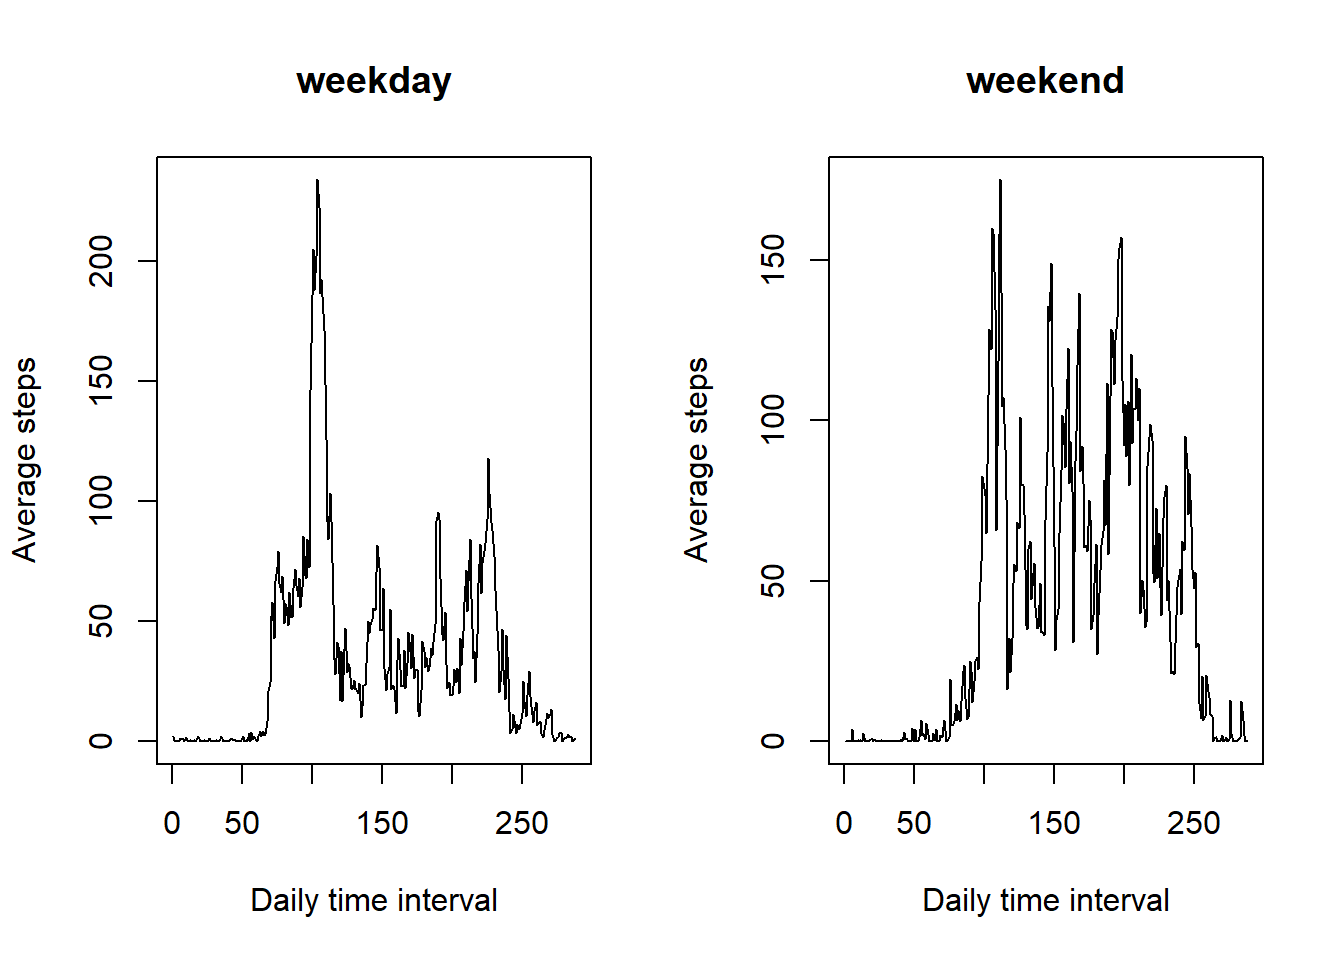
\includegraphics{PA1_template.Rmd_files/figure-latex/weekday_plot-1.pdf}

\begin{Shaded}
\begin{Highlighting}[]
\KeywordTok{par}\NormalTok{(}\DataTypeTok{mfrow=}\KeywordTok{c}\NormalTok{(}\DecValTok{1}\NormalTok{,}\DecValTok{1}\NormalTok{))}
\end{Highlighting}
\end{Shaded}

\end{document}
